\documentclass[10pt,letterpaper,twocolumn]{article} 
\usepackage[margin=1in]{geometry}
\usepackage{minted}
\usepackage{pslatex}
\usepackage{graphicx}
\usepackage{wrapfig}
\usepackage{dblfloatfix}
\usepackage{url}
\newcommand{\figref}[1]{Figure~\ref{fig:#1}}
\newcommand{\punt}[1]{}

%\usepackage{titling}             % Uncomment both to   
%\setlength{\droptitle}{-2em}     % change title position 

\begin{document}
\special{papersize=8.5in,11in}% Still need this even with letterpaper
\title{SuperMalloc: A Super Fast Multithreaded \texttt{malloc()} for HTM}
\author{Bradley C. Kuszmaul \hspace{0.2in} \texttt{bradley@mit.edu}}
\date{}
\vskip -2em
\maketitle
\vskip -1.5em

SuperMalloc is an implementation of \texttt{malloc(3)} designed for
x86 Hardware Transactional Memory (HTM).  It turns out that the same
design also makes it fast even without HTM.  On high-threadcount
workloads on Sandy Bridge (non-HTM) hardware, SuperMalloc outperforms
the competition by about a factor of 3.5.

{\bf Background:} DLmalloc~\cite{Lea96} is the single-threaded
allocator shipped with Linux.  It is simple and has been stable for
decades.  Hoard~\cite{BergerMcBl00} was an early multithreaded
allocators, and provided provable bounds on its space blowup.  In my
experience, JEmalloc~\cite{Evans06} is the best allocator out there.
JEmalloc is ships with BSD and Mozilla.  JEmalloc strives to minimize
footprint in long-running processes such as browsers and database
servers.

{\bf Performance:} \figref{data} compares the performance of
SuperMalloc against DLmalloc, Hoard, and JEmalloc on the malloc-test
benchmark~\cite{LeverBo00}.  The malloc-test benchmark runs $K$
producer threads and $K$ consumer threads.  Each producer thread
allocates objects as fast as possible, and each consumer frees them.
Malloc-test offers one of the most difficult workloads for
multithreaded allocators that employ per-thread caching, since the
per-thread caches can quickly become unbalanced.


{\bf How they work:} DLmalloc~\cite{Lea96} employs boundary tags for
each object, which contributes to space overhead for small objects,
and uses a first-fit heuristic.  DLmalloc has no per-thread caching.
The others allocate large aligned chunks which contain objects that
are all the same size, and provide per-thread caches.

The chunk-based allocators each maintain a table which, given a chunk,
provides the size of that chunk's objects.  One SuperMalloc innovation
is to use an array to implement that table instead of a tree. Since
the usable address space is $2^{48}$ bytes and chunks are $2^{21}$
bytes, there are only $2^{27}$ entries in the table.  The SuperMalloc
table consumes $512$MiB of virtual address space, but since the
operating system provides a lazy page-allocation strategy, the system
typically allocates only a few of pages physical memory.  One design
principle for 64-bit software is ``it is OK to waste some virtual
address space.''

\begin{figure}
% GNUPLOT: LaTeX picture with Postscript
\begingroup
  \fontfamily{ptm}%
  \selectfont
  \makeatletter
  \providecommand\color[2][]{%
    \GenericError{(gnuplot) \space\space\space\@spaces}{%
      Package color not loaded in conjunction with
      terminal option `colourtext'%
    }{See the gnuplot documentation for explanation.%
    }{Either use 'blacktext' in gnuplot or load the package
      color.sty in LaTeX.}%
    \renewcommand\color[2][]{}%
  }%
  \providecommand\includegraphics[2][]{%
    \GenericError{(gnuplot) \space\space\space\@spaces}{%
      Package graphicx or graphics not loaded%
    }{See the gnuplot documentation for explanation.%
    }{The gnuplot epslatex terminal needs graphicx.sty or graphics.sty.}%
    \renewcommand\includegraphics[2][]{}%
  }%
  \providecommand\rotatebox[2]{#2}%
  \@ifundefined{ifGPcolor}{%
    \newif\ifGPcolor
    \GPcolortrue
  }{}%
  \@ifundefined{ifGPblacktext}{%
    \newif\ifGPblacktext
    \GPblacktextfalse
  }{}%
  % define a \g@addto@macro without @ in the name:
  \let\gplgaddtomacro\g@addto@macro
  % define empty templates for all commands taking text:
  \gdef\gplbacktext{}%
  \gdef\gplfronttext{}%
  \makeatother
  \ifGPblacktext
    % no textcolor at all
    \def\colorrgb#1{}%
    \def\colorgray#1{}%
  \else
    % gray or color?
    \ifGPcolor
      \def\colorrgb#1{\color[rgb]{#1}}%
      \def\colorgray#1{\color[gray]{#1}}%
      \expandafter\def\csname LTw\endcsname{\color{white}}%
      \expandafter\def\csname LTb\endcsname{\color{black}}%
      \expandafter\def\csname LTa\endcsname{\color{black}}%
      \expandafter\def\csname LT0\endcsname{\color[rgb]{1,0,0}}%
      \expandafter\def\csname LT1\endcsname{\color[rgb]{0,1,0}}%
      \expandafter\def\csname LT2\endcsname{\color[rgb]{0,0,1}}%
      \expandafter\def\csname LT3\endcsname{\color[rgb]{1,0,1}}%
      \expandafter\def\csname LT4\endcsname{\color[rgb]{0,1,1}}%
      \expandafter\def\csname LT5\endcsname{\color[rgb]{1,1,0}}%
      \expandafter\def\csname LT6\endcsname{\color[rgb]{0,0,0}}%
      \expandafter\def\csname LT7\endcsname{\color[rgb]{1,0.3,0}}%
      \expandafter\def\csname LT8\endcsname{\color[rgb]{0.5,0.5,0.5}}%
    \else
      % gray
      \def\colorrgb#1{\color{black}}%
      \def\colorgray#1{\color[gray]{#1}}%
      \expandafter\def\csname LTw\endcsname{\color{white}}%
      \expandafter\def\csname LTb\endcsname{\color{black}}%
      \expandafter\def\csname LTa\endcsname{\color{black}}%
      \expandafter\def\csname LT0\endcsname{\color{black}}%
      \expandafter\def\csname LT1\endcsname{\color{black}}%
      \expandafter\def\csname LT2\endcsname{\color{black}}%
      \expandafter\def\csname LT3\endcsname{\color{black}}%
      \expandafter\def\csname LT4\endcsname{\color{black}}%
      \expandafter\def\csname LT5\endcsname{\color{black}}%
      \expandafter\def\csname LT6\endcsname{\color{black}}%
      \expandafter\def\csname LT7\endcsname{\color{black}}%
      \expandafter\def\csname LT8\endcsname{\color{black}}%
    \fi
  \fi
  \setlength{\unitlength}{0.0500bp}%
  \begin{picture}(5760.00,3240.00)%
    \gplgaddtomacro\gplbacktext{%
      \csname LTb\endcsname%
      \put(640,558){\makebox(0,0)[r]{\strut{}\footnotesize 0}}%
      \csname LTb\endcsname%
      \put(640,1482){\makebox(0,0)[r]{\strut{}\footnotesize$50$M}}%
      \csname LTb\endcsname%
      \put(640,2407){\makebox(0,0)[r]{\strut{}\footnotesize$100$M}}%
      \csname LTb\endcsname%
      \put(640,2998){\makebox(0,0)[r]{\strut{}\footnotesize $132$M}}%
      \csname LTb\endcsname%
      \put(969,298){\makebox(0,0){\strut{} 1}}%
      \csname LTb\endcsname%
      \put(2036,298){\makebox(0,0){\strut{} 8}}%
      \csname LTb\endcsname%
      \put(3257,298){\makebox(0,0){\strut{} 16}}%
      \csname LTb\endcsname%
      \put(4477,298){\makebox(0,0){\strut{} 24}}%
      \csname LTb\endcsname%
      \put(5698,298){\makebox(0,0){\strut{} 32}}%
      \csname LTb\endcsname%
      \put(37,1796){\rotatebox{-270}{\makebox(0,0){\small \texttt{malloc()}'s per second}}}%
      \csname LTb\endcsname%
      \put(3287,19){\makebox(0,0){\small Producer threads}}%
      \put(3287,2942){\makebox(0,0){\strut{}}}%
      \csname LTb\endcsname%
      \put(3287,2941){\makebox(0,0){\strut{}}}%
      \colorrgb{0.00,0.39,0.00}%
      \put(3104,2776){\makebox(0,0)[r]{\strut{}\footnotesize SuperMalloc}}%
      \colorrgb{0.63,0.00,0.00}%
      \put(3562,669){\makebox(0,0)[r]{\strut{}\footnotesize DLmalloc}}%
      \colorrgb{0.63,0.00,0.63}%
      \put(5698,1575){\makebox(0,0)[r]{\strut{}\footnotesize Hoard}}%
      \colorrgb{0.00,0.00,0.63}%
      \put(3867,1575){\makebox(0,0){\strut{}\footnotesize JEmalloc}}%
      \colorrgb{0.00,0.63,0.63}%
      \put(3104,1390){\makebox(0,0)[r]{\strut{}\footnotesize TBBmalloc}}%
    }%
    \gplgaddtomacro\gplfronttext{%
    }%
    \gplbacktext
    \put(0,0){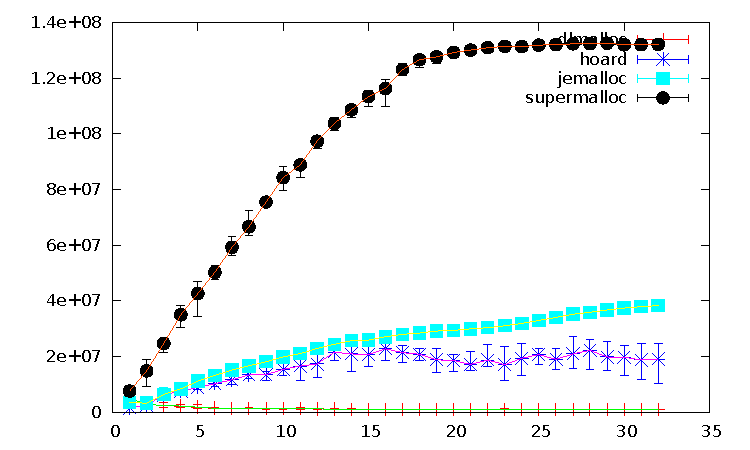
\includegraphics{new-malloc-test-1K-tempo-aggregated}}%
    \gplfronttext
  \end{picture}%
\endgroup

\caption{A comparison of SuperMalloc, DLmalloc \cite{Lea96}, Hoard
  \cite{BergerMcBl00}, and JEmalloc~\cite{Evans06} running malloc-test
  on a 16-core (2 sockets + hyperthreading) 2.4GHz E5-2665 (Sandy
  Bridge).  The lines are the average of 8 trials, and the error bars
  show the fastest and slow trial.}
\label{fig:data}
\vspace*{-3ex}
\end{figure}

%SuperMalloc uses simple data structures to try to maximize the odds that hardware transactions succeed. For example, the SuperMalloc uses a priority heap to allocate objects out of the fullest page. The heap takes advantage of the fact that for each class, there are only a relatively small number of possible page-fullness values. For example, for 8-byte objects, there are only 512 objects in a page, and so instead of using a general heap, SuperMalloc uses an array of 513 lists, the $i$th list containing a list of pages with $i$ free slots.

A second innovation is to employ a per-CPU cache, in addition to a
per-thread cache.  The cost of locking and accessing a shared data
structure turns out to be mostly due to cache coherence traffic from
accessing the object, rather than the locking instructions.  E.g., on
our 2-socket machine, locking and accessing a contended object costs
$460$ns.  Locking and accessing an uncontended object (one that was
last accessed on the same processor) costs only 26ns.  Accessing a
thread-local object with no locking costs $3$ns.  The SuperMalloc
per-thread cache contains just enough objects to amortize the $23$ns
uncontended locking overhead.  The per-CPU cache contains just enough
objects in each class to fill up the hardware cache, the rationale
being that if the working set of a thread is bigger than the hardware
cache, there is no point in working hard to avoid a few more cache
misses.  In contrast, the other allocators may have many megabytes in
their per-thread caches (and because there are many per-thread caches,
their footprint is larger.)  Thus, a second design principle is
``uncontended locking is not so bad''.


%SuperMalloc uses a per-CPU cache and a per-thread cache. A per-thread cache of objects reduces the overhead of allocating and freeing objects because some objects do not need to perform any mutual exclusion. It turns out that most of the cost of updating a global data structure is due to cache misses, not the locking itself, however. On Haswell, an unlocked update to an uncontended cache line costs 3--5ns, whereas acquiring a lock and modifying uncontended variable costs 80ns. Acquiring an uncontended lock and updating an uncontended page costs only about 18ns. (On a multisocket Sandy Bridge processor, the difference is even more striking: 3ns uncontended unlocked, 26ns uncontended locked, and 460ns contended locked.) Accordingly, SuperMalloc uses a relatively small per-thread cache (containing only a few objects of each size), and uses a per-CPU cache (a cache per hardware thread). The per-CPU cache contains only one L3-cache worth of objects for each size class, since we assume that the application will actually store data into allocated objects. If the objects in the per-CPU cache don't fit in the L3 cache, then filling the objects will cause cache misses anyway, so it does not matter whether allocating the objects causes a few cache misses.

% To further improve the odds of transactions committing, SuperMalloc tries to prefetch into cache all the data of the transaction. Prefetching data appears to improve performance by about 5%.

%SuperMalloc appears to enjoy a substantially smaller footprint than the other allocators for two reasons. (1) SuperMalloc adopts Hoard's allocate-in-fullest-page heuristic rather than JEmalloc's approach of allocating the object with the lowest address. (2) SuperMalloc's caches are smaller than Hoard's or JEmallocs, mostly because the per-thread cache is extremely small, and in many applications there are far more threads than there are CPU's.

% SuperMalloc is currently implemented, and we are assembling and running the allocation benchmarks mentioned in other allocation papers. We plan to release the software under the Apache 2.0 license, and the assembled benchmarks under an appropriate mix of licenses.

SuperMalloc, like Hoard, allocates objects out of the fullest possible page in order to reduce memory footprint.

I will soon release SuperMalloc under an open-source license.

{
\let\oldbibliography\thebibliography
\renewcommand{\thebibliography}[1]{%
  \oldbibliography{#1}%
  \setlength{\itemsep}{0pt}%
}
\footnotesize
\bibliographystyle{abbrv-url}
\bibliography{allpapers}
}

%% \begin{figure*}
%% \begin{tabular}{cc}
%% % GNUPLOT: LaTeX picture with Postscript
\begingroup
  \fontfamily{ptm}%
  \selectfont
  \makeatletter
  \providecommand\color[2][]{%
    \GenericError{(gnuplot) \space\space\space\@spaces}{%
      Package color not loaded in conjunction with
      terminal option `colourtext'%
    }{See the gnuplot documentation for explanation.%
    }{Either use 'blacktext' in gnuplot or load the package
      color.sty in LaTeX.}%
    \renewcommand\color[2][]{}%
  }%
  \providecommand\includegraphics[2][]{%
    \GenericError{(gnuplot) \space\space\space\@spaces}{%
      Package graphicx or graphics not loaded%
    }{See the gnuplot documentation for explanation.%
    }{The gnuplot epslatex terminal needs graphicx.sty or graphics.sty.}%
    \renewcommand\includegraphics[2][]{}%
  }%
  \providecommand\rotatebox[2]{#2}%
  \@ifundefined{ifGPcolor}{%
    \newif\ifGPcolor
    \GPcolortrue
  }{}%
  \@ifundefined{ifGPblacktext}{%
    \newif\ifGPblacktext
    \GPblacktextfalse
  }{}%
  % define a \g@addto@macro without @ in the name:
  \let\gplgaddtomacro\g@addto@macro
  % define empty templates for all commands taking text:
  \gdef\gplbacktext{}%
  \gdef\gplfronttext{}%
  \makeatother
  \ifGPblacktext
    % no textcolor at all
    \def\colorrgb#1{}%
    \def\colorgray#1{}%
  \else
    % gray or color?
    \ifGPcolor
      \def\colorrgb#1{\color[rgb]{#1}}%
      \def\colorgray#1{\color[gray]{#1}}%
      \expandafter\def\csname LTw\endcsname{\color{white}}%
      \expandafter\def\csname LTb\endcsname{\color{black}}%
      \expandafter\def\csname LTa\endcsname{\color{black}}%
      \expandafter\def\csname LT0\endcsname{\color[rgb]{1,0,0}}%
      \expandafter\def\csname LT1\endcsname{\color[rgb]{0,1,0}}%
      \expandafter\def\csname LT2\endcsname{\color[rgb]{0,0,1}}%
      \expandafter\def\csname LT3\endcsname{\color[rgb]{1,0,1}}%
      \expandafter\def\csname LT4\endcsname{\color[rgb]{0,1,1}}%
      \expandafter\def\csname LT5\endcsname{\color[rgb]{1,1,0}}%
      \expandafter\def\csname LT6\endcsname{\color[rgb]{0,0,0}}%
      \expandafter\def\csname LT7\endcsname{\color[rgb]{1,0.3,0}}%
      \expandafter\def\csname LT8\endcsname{\color[rgb]{0.5,0.5,0.5}}%
    \else
      % gray
      \def\colorrgb#1{\color{black}}%
      \def\colorgray#1{\color[gray]{#1}}%
      \expandafter\def\csname LTw\endcsname{\color{white}}%
      \expandafter\def\csname LTb\endcsname{\color{black}}%
      \expandafter\def\csname LTa\endcsname{\color{black}}%
      \expandafter\def\csname LT0\endcsname{\color{black}}%
      \expandafter\def\csname LT1\endcsname{\color{black}}%
      \expandafter\def\csname LT2\endcsname{\color{black}}%
      \expandafter\def\csname LT3\endcsname{\color{black}}%
      \expandafter\def\csname LT4\endcsname{\color{black}}%
      \expandafter\def\csname LT5\endcsname{\color{black}}%
      \expandafter\def\csname LT6\endcsname{\color{black}}%
      \expandafter\def\csname LT7\endcsname{\color{black}}%
      \expandafter\def\csname LT8\endcsname{\color{black}}%
    \fi
  \fi
  \setlength{\unitlength}{0.0500bp}%
  \begin{picture}(5760.00,3240.00)%
    \gplgaddtomacro\gplbacktext{%
      \csname LTb\endcsname%
      \put(640,558){\makebox(0,0)[r]{\strut{}\footnotesize 0}}%
      \csname LTb\endcsname%
      \put(640,1482){\makebox(0,0)[r]{\strut{}\footnotesize$50$M}}%
      \csname LTb\endcsname%
      \put(640,2407){\makebox(0,0)[r]{\strut{}\footnotesize$100$M}}%
      \csname LTb\endcsname%
      \put(640,2998){\makebox(0,0)[r]{\strut{}\footnotesize $132$M}}%
      \csname LTb\endcsname%
      \put(969,298){\makebox(0,0){\strut{} 1}}%
      \csname LTb\endcsname%
      \put(2036,298){\makebox(0,0){\strut{} 8}}%
      \csname LTb\endcsname%
      \put(3257,298){\makebox(0,0){\strut{} 16}}%
      \csname LTb\endcsname%
      \put(4477,298){\makebox(0,0){\strut{} 24}}%
      \csname LTb\endcsname%
      \put(5698,298){\makebox(0,0){\strut{} 32}}%
      \csname LTb\endcsname%
      \put(37,1796){\rotatebox{-270}{\makebox(0,0){\small \texttt{malloc()}'s per second}}}%
      \csname LTb\endcsname%
      \put(3287,19){\makebox(0,0){\small Producer threads}}%
      \put(3287,2942){\makebox(0,0){\strut{}}}%
      \csname LTb\endcsname%
      \put(3287,2941){\makebox(0,0){\strut{}}}%
      \colorrgb{0.00,0.39,0.00}%
      \put(3104,2776){\makebox(0,0)[r]{\strut{}\footnotesize SuperMalloc}}%
      \colorrgb{0.63,0.00,0.00}%
      \put(3562,669){\makebox(0,0)[r]{\strut{}\footnotesize DLmalloc}}%
      \colorrgb{0.63,0.00,0.63}%
      \put(5698,1575){\makebox(0,0)[r]{\strut{}\footnotesize Hoard}}%
      \colorrgb{0.00,0.00,0.63}%
      \put(3867,1575){\makebox(0,0){\strut{}\footnotesize JEmalloc}}%
      \colorrgb{0.00,0.63,0.63}%
      \put(3104,1390){\makebox(0,0)[r]{\strut{}\footnotesize TBBmalloc}}%
    }%
    \gplgaddtomacro\gplfronttext{%
    }%
    \gplbacktext
    \put(0,0){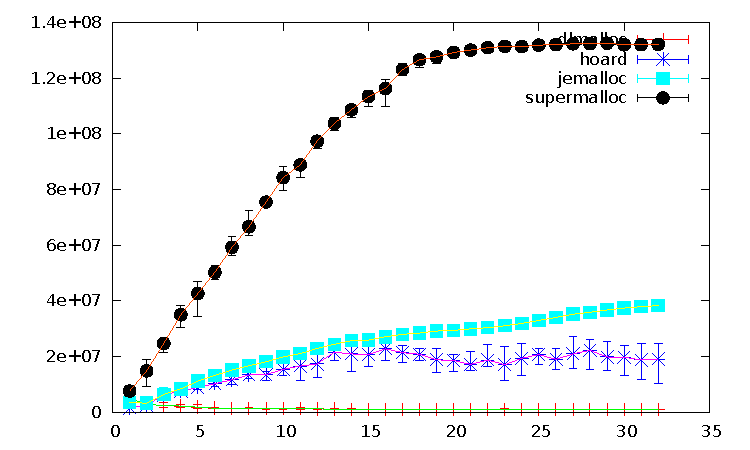
\includegraphics{new-malloc-test-1K-tempo-aggregated}}%
    \gplfronttext
  \end{picture}%
\endgroup

%% &
%% % GNUPLOT: LaTeX picture with Postscript
\begingroup
  \fontfamily{ptm}%
  \selectfont
  \makeatletter
  \providecommand\color[2][]{%
    \GenericError{(gnuplot) \space\space\space\@spaces}{%
      Package color not loaded in conjunction with
      terminal option `colourtext'%
    }{See the gnuplot documentation for explanation.%
    }{Either use 'blacktext' in gnuplot or load the package
      color.sty in LaTeX.}%
    \renewcommand\color[2][]{}%
  }%
  \providecommand\includegraphics[2][]{%
    \GenericError{(gnuplot) \space\space\space\@spaces}{%
      Package graphicx or graphics not loaded%
    }{See the gnuplot documentation for explanation.%
    }{The gnuplot epslatex terminal needs graphicx.sty or graphics.sty.}%
    \renewcommand\includegraphics[2][]{}%
  }%
  \providecommand\rotatebox[2]{#2}%
  \@ifundefined{ifGPcolor}{%
    \newif\ifGPcolor
    \GPcolortrue
  }{}%
  \@ifundefined{ifGPblacktext}{%
    \newif\ifGPblacktext
    \GPblacktextfalse
  }{}%
  % define a \g@addto@macro without @ in the name:
  \let\gplgaddtomacro\g@addto@macro
  % define empty templates for all commands taking text:
  \gdef\gplbacktext{}%
  \gdef\gplfronttext{}%
  \makeatother
  \ifGPblacktext
    % no textcolor at all
    \def\colorrgb#1{}%
    \def\colorgray#1{}%
  \else
    % gray or color?
    \ifGPcolor
      \def\colorrgb#1{\color[rgb]{#1}}%
      \def\colorgray#1{\color[gray]{#1}}%
      \expandafter\def\csname LTw\endcsname{\color{white}}%
      \expandafter\def\csname LTb\endcsname{\color{black}}%
      \expandafter\def\csname LTa\endcsname{\color{black}}%
      \expandafter\def\csname LT0\endcsname{\color[rgb]{1,0,0}}%
      \expandafter\def\csname LT1\endcsname{\color[rgb]{0,1,0}}%
      \expandafter\def\csname LT2\endcsname{\color[rgb]{0,0,1}}%
      \expandafter\def\csname LT3\endcsname{\color[rgb]{1,0,1}}%
      \expandafter\def\csname LT4\endcsname{\color[rgb]{0,1,1}}%
      \expandafter\def\csname LT5\endcsname{\color[rgb]{1,1,0}}%
      \expandafter\def\csname LT6\endcsname{\color[rgb]{0,0,0}}%
      \expandafter\def\csname LT7\endcsname{\color[rgb]{1,0.3,0}}%
      \expandafter\def\csname LT8\endcsname{\color[rgb]{0.5,0.5,0.5}}%
    \else
      % gray
      \def\colorrgb#1{\color{black}}%
      \def\colorgray#1{\color[gray]{#1}}%
      \expandafter\def\csname LTw\endcsname{\color{white}}%
      \expandafter\def\csname LTb\endcsname{\color{black}}%
      \expandafter\def\csname LTa\endcsname{\color{black}}%
      \expandafter\def\csname LT0\endcsname{\color{black}}%
      \expandafter\def\csname LT1\endcsname{\color{black}}%
      \expandafter\def\csname LT2\endcsname{\color{black}}%
      \expandafter\def\csname LT3\endcsname{\color{black}}%
      \expandafter\def\csname LT4\endcsname{\color{black}}%
      \expandafter\def\csname LT5\endcsname{\color{black}}%
      \expandafter\def\csname LT6\endcsname{\color{black}}%
      \expandafter\def\csname LT7\endcsname{\color{black}}%
      \expandafter\def\csname LT8\endcsname{\color{black}}%
    \fi
  \fi
  \setlength{\unitlength}{0.0500bp}%
  \begin{picture}(4320.00,2720.00)%
    \gplgaddtomacro\gplbacktext{%
      \csname LTb\endcsname%
      \put(538,558){\makebox(0,0)[r]{\strut{}\footnotesize 0}}%
      \csname LTb\endcsname%
      \put(538,1156){\makebox(0,0)[r]{\strut{}\footnotesize $50$M}}%
      \csname LTb\endcsname%
      \put(538,1694){\makebox(0,0)[r]{\strut{}\footnotesize $95$M}}%
      \csname LTb\endcsname%
      \put(809,298){\makebox(0,0){\strut{} 1}}%
      \csname LTb\endcsname%
      \put(1283,298){\makebox(0,0){\strut{} 2}}%
      \csname LTb\endcsname%
      \put(1758,298){\makebox(0,0){\strut{} 3}}%
      \csname LTb\endcsname%
      \put(2232,298){\makebox(0,0){\strut{} 4}}%
      \csname LTb\endcsname%
      \put(2706,298){\makebox(0,0){\strut{} 5}}%
      \csname LTb\endcsname%
      \put(3181,298){\makebox(0,0){\strut{} 6}}%
      \csname LTb\endcsname%
      \put(3655,298){\makebox(0,0){\strut{} 7}}%
      \csname LTb\endcsname%
      \put(4129,298){\makebox(0,0){\strut{} 8}}%
      \csname LTb\endcsname%
      \put(88,1359){\rotatebox{-270}{\makebox(0,0){\small \texttt{malloc()}'s per second}}}%
      \csname LTb\endcsname%
      \put(2516,19){\makebox(0,0){\small Producer threads}}%
      \put(2516,2440){\makebox(0,0){\strut{}\small 4-Core (8 hardware threads) 3.4GHz Haswell}}%
      \csname LTb\endcsname%
      \put(2516,2067){\makebox(0,0){\strut{}}}%
      \colorrgb{0.00,0.39,0.00}%
      \put(2090,1515){\makebox(0,0)[r]{\strut{}\footnotesize SuperMalloc}}%
      \colorrgb{0.63,0.00,0.00}%
      \put(2706,644){\makebox(0,0)[r]{\strut{}\footnotesize dlmalloc}}%
      \colorrgb{0.00,0.00,0.63}%
      \put(4082,678){\makebox(0,0)[r]{\strut{}\footnotesize Hoard}}%
      \colorrgb{0.63,0.00,0.63}%
      \put(4129,989){\makebox(0,0)[r]{\strut{}\footnotesize jemalloc}}%
    }%
    \gplgaddtomacro\gplfronttext{%
    }%
    \gplbacktext
    \put(0,0){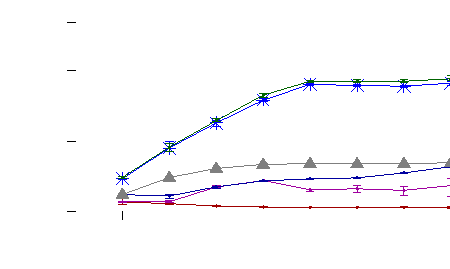
\includegraphics{new-malloc-test-1K-lutestring-aggregated}}%
    \gplfronttext
  \end{picture}%
\endgroup

%% \end{tabular}
%% \caption{A comparison of SuperMalloc, dlmalloc, Hoard, and jemalloc on the malloc-test benchmark.}
%% \label{fig:data}
%% \end{figure*}

\end{document}

%%  LocalWords:  SuperMalloc Transactional threadcount multithreaded
%%  LocalWords:  allocator allocators JEmalloc HTM DLmalloc malloc ns
%%  LocalWords:  uncontended
